%%%%%%%%%%%%%%%%%%%%%%%%%%%%%%
% Ioannis Petrousov
% petrousov@gmail.com
% 2025
%
% Custom Latex thesis template
% to be used for English language.
%
% Initial compile:
%     1. xelatex
%     2. bibtex
%     3. xelatex
%     4. xelatex
%
% Further compile:
%
% A: If you change the bibliography file
%     1. biblatex
%     2. xelatex
%     3. xelatex
%
% B: If you DONT change the bibliography file
%     1. xelatex
%     2. xelatex
%%%%%%%%%%%%%%%%%%%%%%%%%%%%%%

% Use the following documentclass declaration if you plan to make a hardcopy
% The twoside option shift text for making a book print
%\documentclass[12pt,twoside]{report}

% Use the following documentclass for PDF and to view on computer only
\documentclass[8pt,a4paper]{report}%{book}

\usepackage{listings}
\usepackage{csquotes}

\usepackage{float}
% TEXT FORMATTING
% set spacing between lines (line spacing)
\usepackage{setspace}
\setstretch{1.5}
% package to customize chapters, sections and subsections style
\usepackage{titlesec}
% chapter title appearance format
\titleformat{\chapter}[display]
{\bfseries\huge}{\chaptertitlename\space}{16pt}{}
% https://www.sharelatex.com/learn/Sections_and_chapters
\titlespacing{\chapter}{0pc}{1.5ex plus .1ex minus .2ex}{5pc}
% section title appearance format
\titleformat{\section}
{\bfseries\large}{\thesection}{14pt}{}
% subsection title appearance format
\titleformat{\subsection}
{\bfseries\normalsize}{\thesubsection}{12pt}{}
% set margins
\usepackage{geometry}
\geometry{left=3cm, right=2cm, top=2.5cm, bottom=2.5cm}
% text justification is fully-justified by default

% xelatex wants fontspec
\usepackage{fontspec}
\usepackage{xltxtra}
% \setmainfont[Mapping=tex-text]{Latin Modern Roman}
\setmainfont[Mapping=tex-text]{XITS}
% package allows to place figures
\usepackage{graphicx}
% put images in images path
\graphicspath{{images/}}
\usepackage{setspace}

% Caption customization
% use this package to set appearance for captions
\usepackage{caption}
% caption size for figures 10pt
\captionsetup[figure]{font=footnotesize,labelfont=footnotesize}
% caption size for tables 10pt and underlined
\usepackage[normalem]{ulem} % Package for underlining
\DeclareCaptionLabelFormat{label_format}{\uline{#1~#2}} % underline label
\DeclareCaptionTextFormat{text_format}{\uline{#1}} % underline text
\DeclareCaptionLabelSeparator{separator_format}{\uline{:~}} % underline separator
%\captionsetup[table]{font=normalsize,labelfont=normalsize,labelformat=label_format,textformat=text_format,labelseparator=separator_format}

% use this package to define custom colors
\usepackage{xcolor}

% create colors
\colorlet{punct}{red!60!black}
\definecolor{background}{HTML}{EEEEEE}
\definecolor{delim}{RGB}{20,105,176}
\colorlet{numb}{magenta!60!black}

% use this package for algorithms
\usepackage{algorithm2e}

% use math package to create equations
\usepackage{amsmath}

% create command for blank page
\usepackage{afterpage}
\newcommand\blankpage{%
    \null
    \thispagestyle{empty}%
    \addtocounter{page}{-1}%
    \newpage}

% add clickable hyperlinks
\usepackage{hyperref}
\hypersetup{
    colorlinks,
    citecolor=black,
    filecolor=black,
    linkcolor=black,
    urlcolor=black
}

% use fancy header and footer
\usepackage{fancyhdr}
\usepackage{blindtext} % to quickly get a full document

% Turn on the style
\pagestyle{fancy}

% Clear the header and footer
\fancyhf{}

% Set the right side of the footer to be the page number
\fancyfoot[R]{\thepage}

% set page number appearance to bottom right
\fancypagestyle{plain}{%
    \renewcommand{\headrulewidth}{0pt}
    \fancyhf{}
    \fancyfoot[R]{\thepage}%
}

\newcommand{\HRule}{\rule{\linewidth}{0.5mm}}

% change the word 'Algorithm' in caption to Algorithm
\renewcommand*{\algorithmcfname}{Algorithm}

% Change "List of Algorithms" to "List of Algorithms"
\renewcommand\listalgorithmcfname{List of Algorithms}

% package to create and customize appendixes (Appendices)
% put appendix title to table of contents (toc)
% Puts a title (e.g., ‘Appendices’) into the document at the point where the appendices environment is begun (page)
\usepackage[toc,page]{appendix}
% Use fancy tables
\usepackage{booktabs}
% change appendix name to Appendices in table of content
\renewcommand{\appendixtocname}{Appendices}
% change appendix name to Appendices in page
\renewcommand{\appendixpagename}{Appendices}

\begin{document}
\begin{titlepage}
\begin{center}

\begin{figure}[h]
\centering


\includegraphics[width=0.4\textwidth]{images/program_logo.png}
\caption*{D.P.M.S.\\ Artificial Intelligence} % Unnumbered text for the specific program
\end{figure}

% Horizontal row of logos
\begin{center}
    % Define a fixed, consistent height for both images (e.g., 2cm)
    % Use minipages to guarantee they are placed side-by-side

    % Left Logo
    \begin{minipage}{0.48\textwidth} % Takes up almost half the line
        \centering
        
\includegraphics[height=2cm]{images/unipi_logo.png}
    \end{minipage}%
    \hfill % This command pushes the two minipages to the far edges of the center environment
    \begin{minipage}{0.48\textwidth} % Takes up almost half the line
        \centering
        
\includegraphics[height=2cm]{images/demokritos_logo.png}
    \end{minipage}
\end{center}

\begin{center}
% leave 2 cm from above text
\vspace{2cm}

\HRule \\[0.4cm]
{\huge Εργασία 1\\}
\HRule \\[0.4cm]
\end{center}

Course: Natural Language Processing - NLP

% put this on the bottom
\vfill
\begin{doublespacing}

{\LARGE
Ioannis Petrousov\\}
\vfill
{\Large \ifcase\month\or January\or February\or March\or April\or May\or June\or July\or August\or September\or October\or November\or December\fi, \number\year}
\end{doublespacing}
\end{center}
\end{titlepage}

% insert blank page after title page
%\afterpage{\blankpage}

% CONTENT
\section*{Α. Tokens, Types, Zipf’s Law}

\subsection*{1}

\begin{table}[H]
\begin{tabular}{|l|l|l|l|}
\hline
                  &  NLTK & spaCy & Bert   \\ \hline
\#tokens          & 93356 & 97152 & 117968 \\ \hline
\#types           & 11017 & 10445 & 8544   \\ \hline
TTR               & 0.1180& 0.1075& 0.0724 \\ \hline
Hapax legomena    & 5615  & 5072  & 2915   \\ \hline
Hapax dislegomena & 1702  & 1659  & 1381   \\ \hline
\end{tabular}
\end{table}

The method which creates the largest vocabulary is the one with the highest \#types count, in this case NLTK. However, it's important to note that while this number is the highest of all other methods, it's not necessary the most accurate. Specifically, \lstinline{word_tokenize()} uses the Punkt sentence tokenization model to splits the text into individual elements. This model uses a word-based tokenization approach which also splits punctuation marks, including ",", "." and "'" into separate tokens thus increasing the \#types count. The same can be observed for the tokenization method \lstinline{spaCy} uses. This results into creating tokens of the form:

\begin{lstlisting}
    In [1]: "." in tokens
    Out[1]: True

    In [2]: "," in tokens
    Out[2]: True

    In [3]: "'" in tokens
    Out[3]: True

    In [4]: "it's" in tokens
    Out[4]: False

    In [5]: "'s" in tokens
    Out[5]: True
\end{lstlisting}

On the other hand, Bert uses a more modern subword tokenization approach - WordPiece. The method effectively recognizes and constructs larger words (from smaller) thus optimizing \#types count.

TTR expresses vocabulary diversity. The higher values observed in NLTK and spaCy indicate a richer vocabulary. However, BERT has a vocabulary consisting of longer words which might have an increased meaning compared to the ones from the aforementioned methods.

Both spaCy and NLTK follow Zipf's law:
$5615/11017=50\%$ and $5072/10445=48\%$ so half of the vocabulary appears only once in the tokens. BERT shows a lower percentage of Hapax Legomena (34\%), likely because its subword units are designed to be highly reusable across different words, reducing the number of unique, single-use types compared to word-based tokenizers.

\subsection*{2}

I selected the first sentence: "Pierre Vinken, 61 years old, will join the board as a nonexecutive director Nov. 29.". Following are the results from the tokenization.

\begin{lstlisting}

    NLTK tokens:
    ['Pierre', 'Vinken', ',', '61', 'years', 'old', ',', 'will',
    'join', 'the', 'board', 'as', 'a', 'nonexecutive', 'director',
    'Nov.', '29', '.']
    ===============
    spaCy tokens:
    ['Pierre', 'Vinken', ',', '61', 'years', 'old', ',', 'will',
    'join', 'the', 'board', 'as', 'a', 'nonexecutive', 'director',
    'Nov.', '29', '.']
    ===============
    BERT tokens:
    ['Pierre', 'Vin', '##ken', ',', '61', 'years', 'old', ',', 'will',
    'join', 'the', 'board', 'as', 'a', 'none', '##xe', '##cut', '##ive',
    'director', 'Nov', '.', '29', '.']
    ===============

\end{lstlisting}

We can see that both NLTK and spaCy managed to split almost all the words correctly because they use a word-based tokenization approach. However, BERT uses a statistical method to construct tokens. In the example we can see that it broke the word "Vinken" into 2: "Vin", "\#\#ken". This happening because the word does not exist in its vocabulary. Also "nonexecutive" was broken into 4 subwords: "none", "\#\#xe", "\#\#cut", and "\#\#ive" because it greedy-matched separate words from it's vocabulary starting with the word "none". It couldn't match the rest of the word ("xecutive") so it broke it into 3 pieces using "\#\#" in front of each piece.

\subsection*{3}

\begin{table}[H]
\begin{tabular}{|c|l|l|l|l|l|l|}
\hline
\multicolumn{1}{|r|}{\textbf{}} & \multicolumn{1}{r|}{\textbf{NLTK Type}} & \multicolumn{1}{r|}{\textbf{NLTK Freq}} & \multicolumn{1}{r|}{\textbf{spaCy Type}} & \multicolumn{1}{r|}{\textbf{spaCy Freq}} & \multicolumn{1}{r|}{\textbf{BERT Type}} & \multicolumn{1}{r|}{\textbf{BERT Freq}} \\ \hline
\textbf{0}                      & ,                                       & 4823                                    & .                                        & 5020                                     & .                                       & 6363                                    \\ \hline
\textbf{1}                      & the                                     & 4757                                    & ,                                        & 4823                                     & ,                                       & 5026                                    \\ \hline
\textbf{2}                      & .                                       & 3645                                    & the                                      & 4763                                     & the                                     & 4767                                    \\ \hline
\textbf{3}                      & of                                      & 2318                                    & of                                       & 2319                                     & '                                       & 4117                                    \\ \hline
\textbf{4}                      & to                                      & 2175                                    & to                                       & 2180                                     & of                                      & 2320                                    \\ \hline
\textbf{5}                      & a                                       & 1967                                    & a                                        & 1991                                     & to                                      & 2226                                    \\ \hline
\textbf{6}                      & in                                      & 1760                                    & in                                       & 1773                                     & a                                       & 2150                                    \\ \hline
\textbf{7}                      & and                                     & 1534                                    & and                                      & 1541                                     & in                                      & 1940                                    \\ \hline
\textbf{8}                      & ''                                      & 959                                     & ''                                       & 1372                                     & -                                       & 1733                                    \\ \hline
\textbf{9}                      & 's                                      & 865                                     & -                                        & 1231                                     & and                                     & 1549                                    \\ \hline
\textbf{10}                     & for                                     & 851                                     & 's                                       & 865                                      & s                                       & 1356                                    \\ \hline
\textbf{11}                     & that                                    & 848                                     & for                                      & 851                                      & for                                     & 870                                     \\ \hline
\textbf{12}                     & \$                                      & 708                                     & NaN                                      & \textless{}NA\textgreater{}              & that                                    & 848                                     \\ \hline
\textbf{13}                     & is                                      & 672                                     & NaN                                      & \textless{}NA\textgreater{}              & NaN                                     & \textless{}NA\textgreater{}             \\ \hline
\end{tabular}
\end{table}

I extracted the number of common tokens programmatically and it was found to be 9. See Python notebook for details.

\subsection*{4}

Following are the optimal calculated values. I used Mean Square Error - MSE to measure the distance between the actual and calculated values for the token appearance frequency.

\begin{table}[H]
\centering
\begin{tabular}{|c|l|l|l|}
\hline
\multicolumn{1}{|r|}{\textbf{}} & \multicolumn{1}{r|}{\textbf{NLTK}} & \multicolumn{1}{r|}{\textbf{spaCy}} & \multicolumn{1}{r|}{\textbf{BERT}} \\ \hline
\textbf{A}                      & 0.1                                & 0.4                                 & 0.1                                \\ \hline
\end{tabular}
\end{table}

\begin{center}
    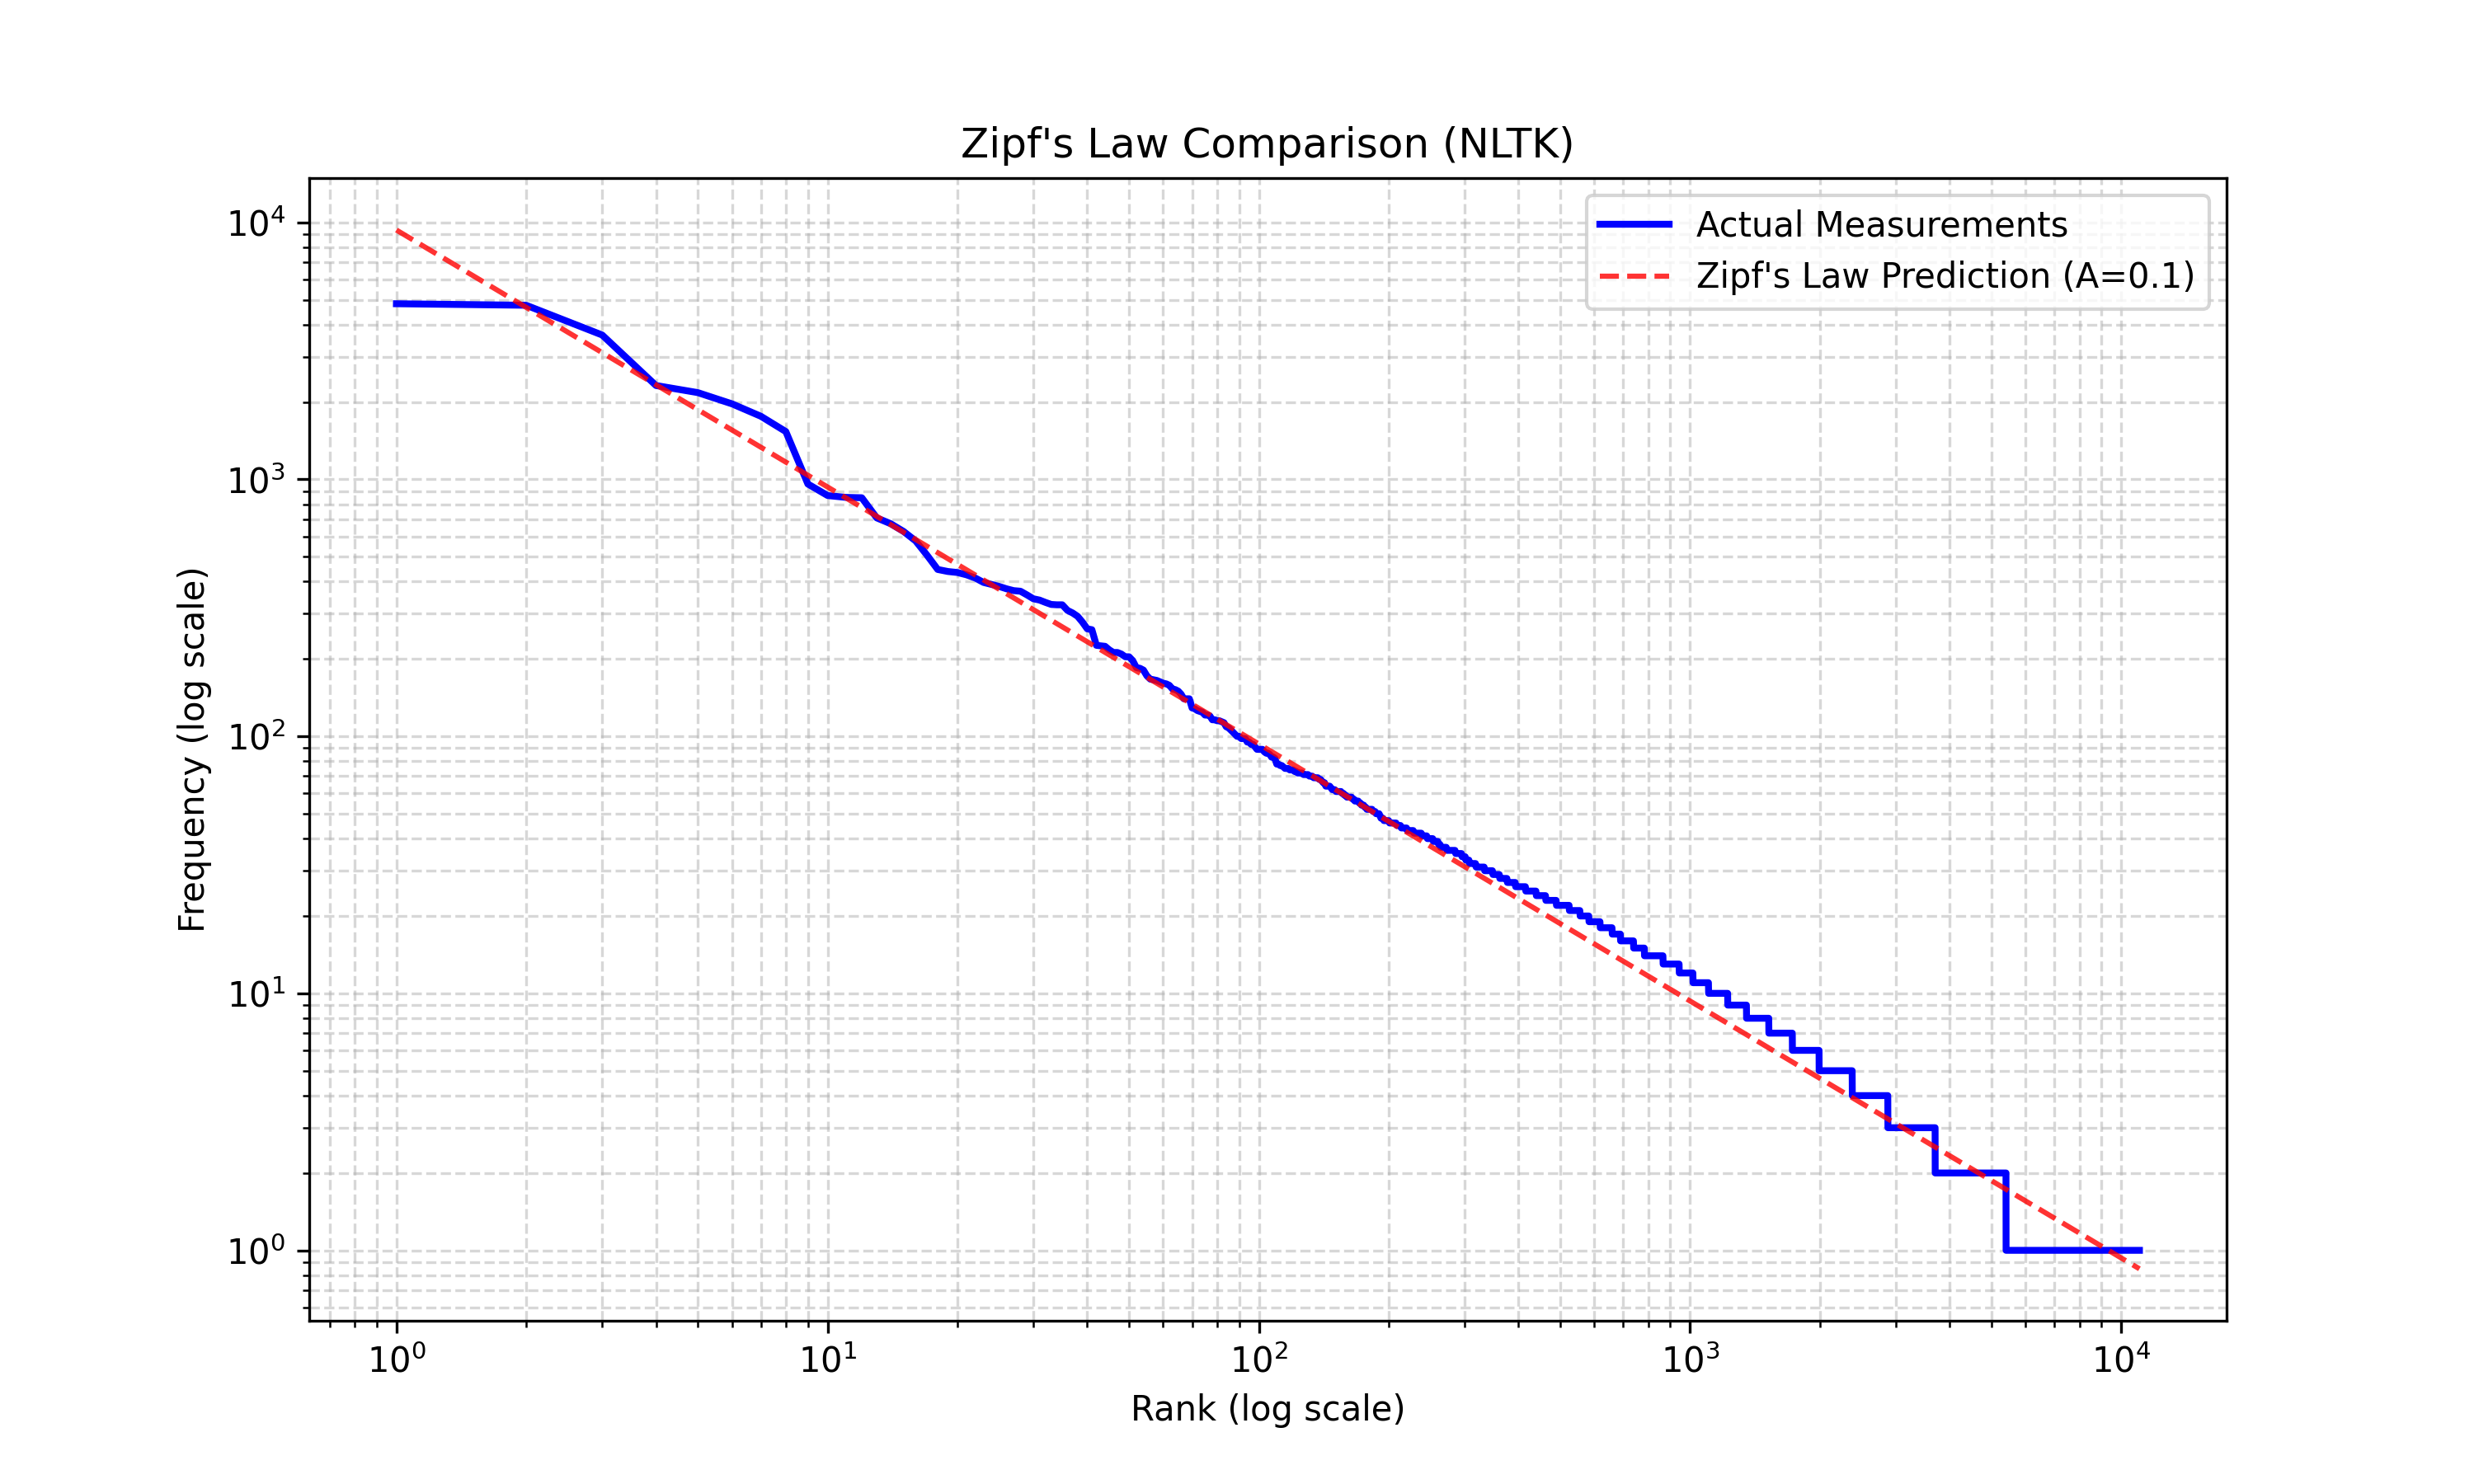
\includegraphics[scale=0.7]{images/nltk_zipf_law_comparison.png}
    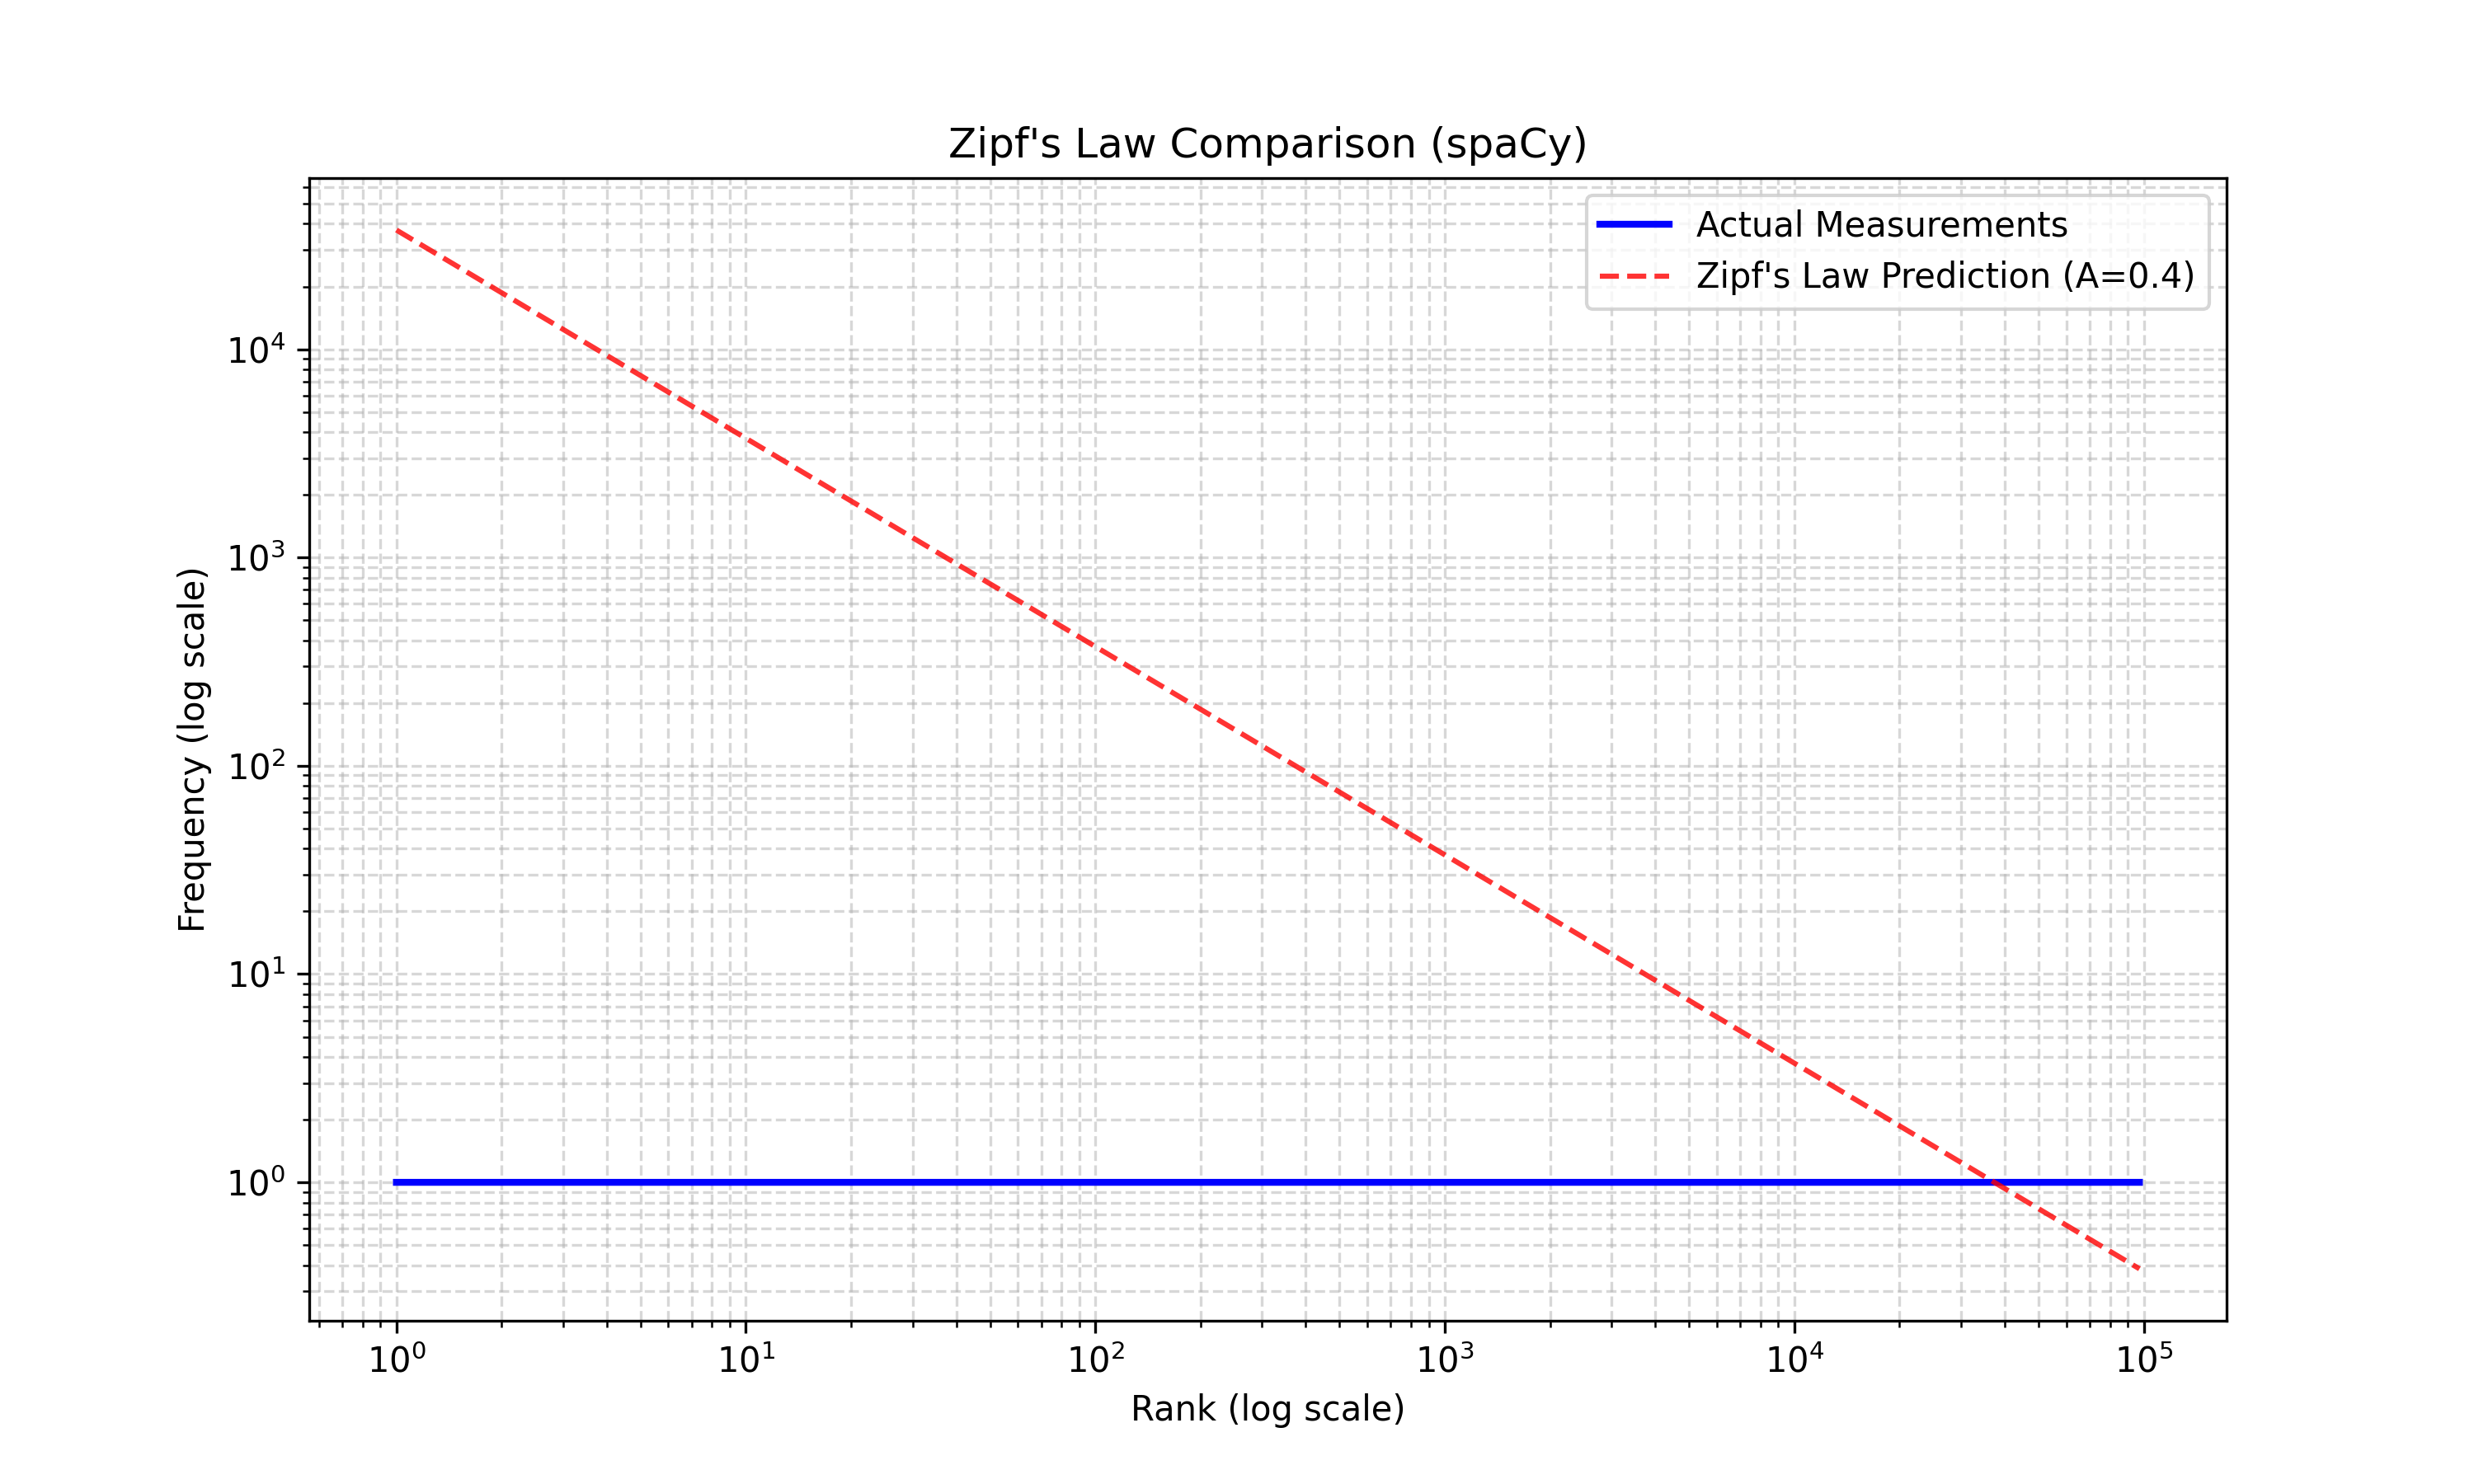
\includegraphics[scale=0.7]{images/spacy_zipf_law_comparison.png}
    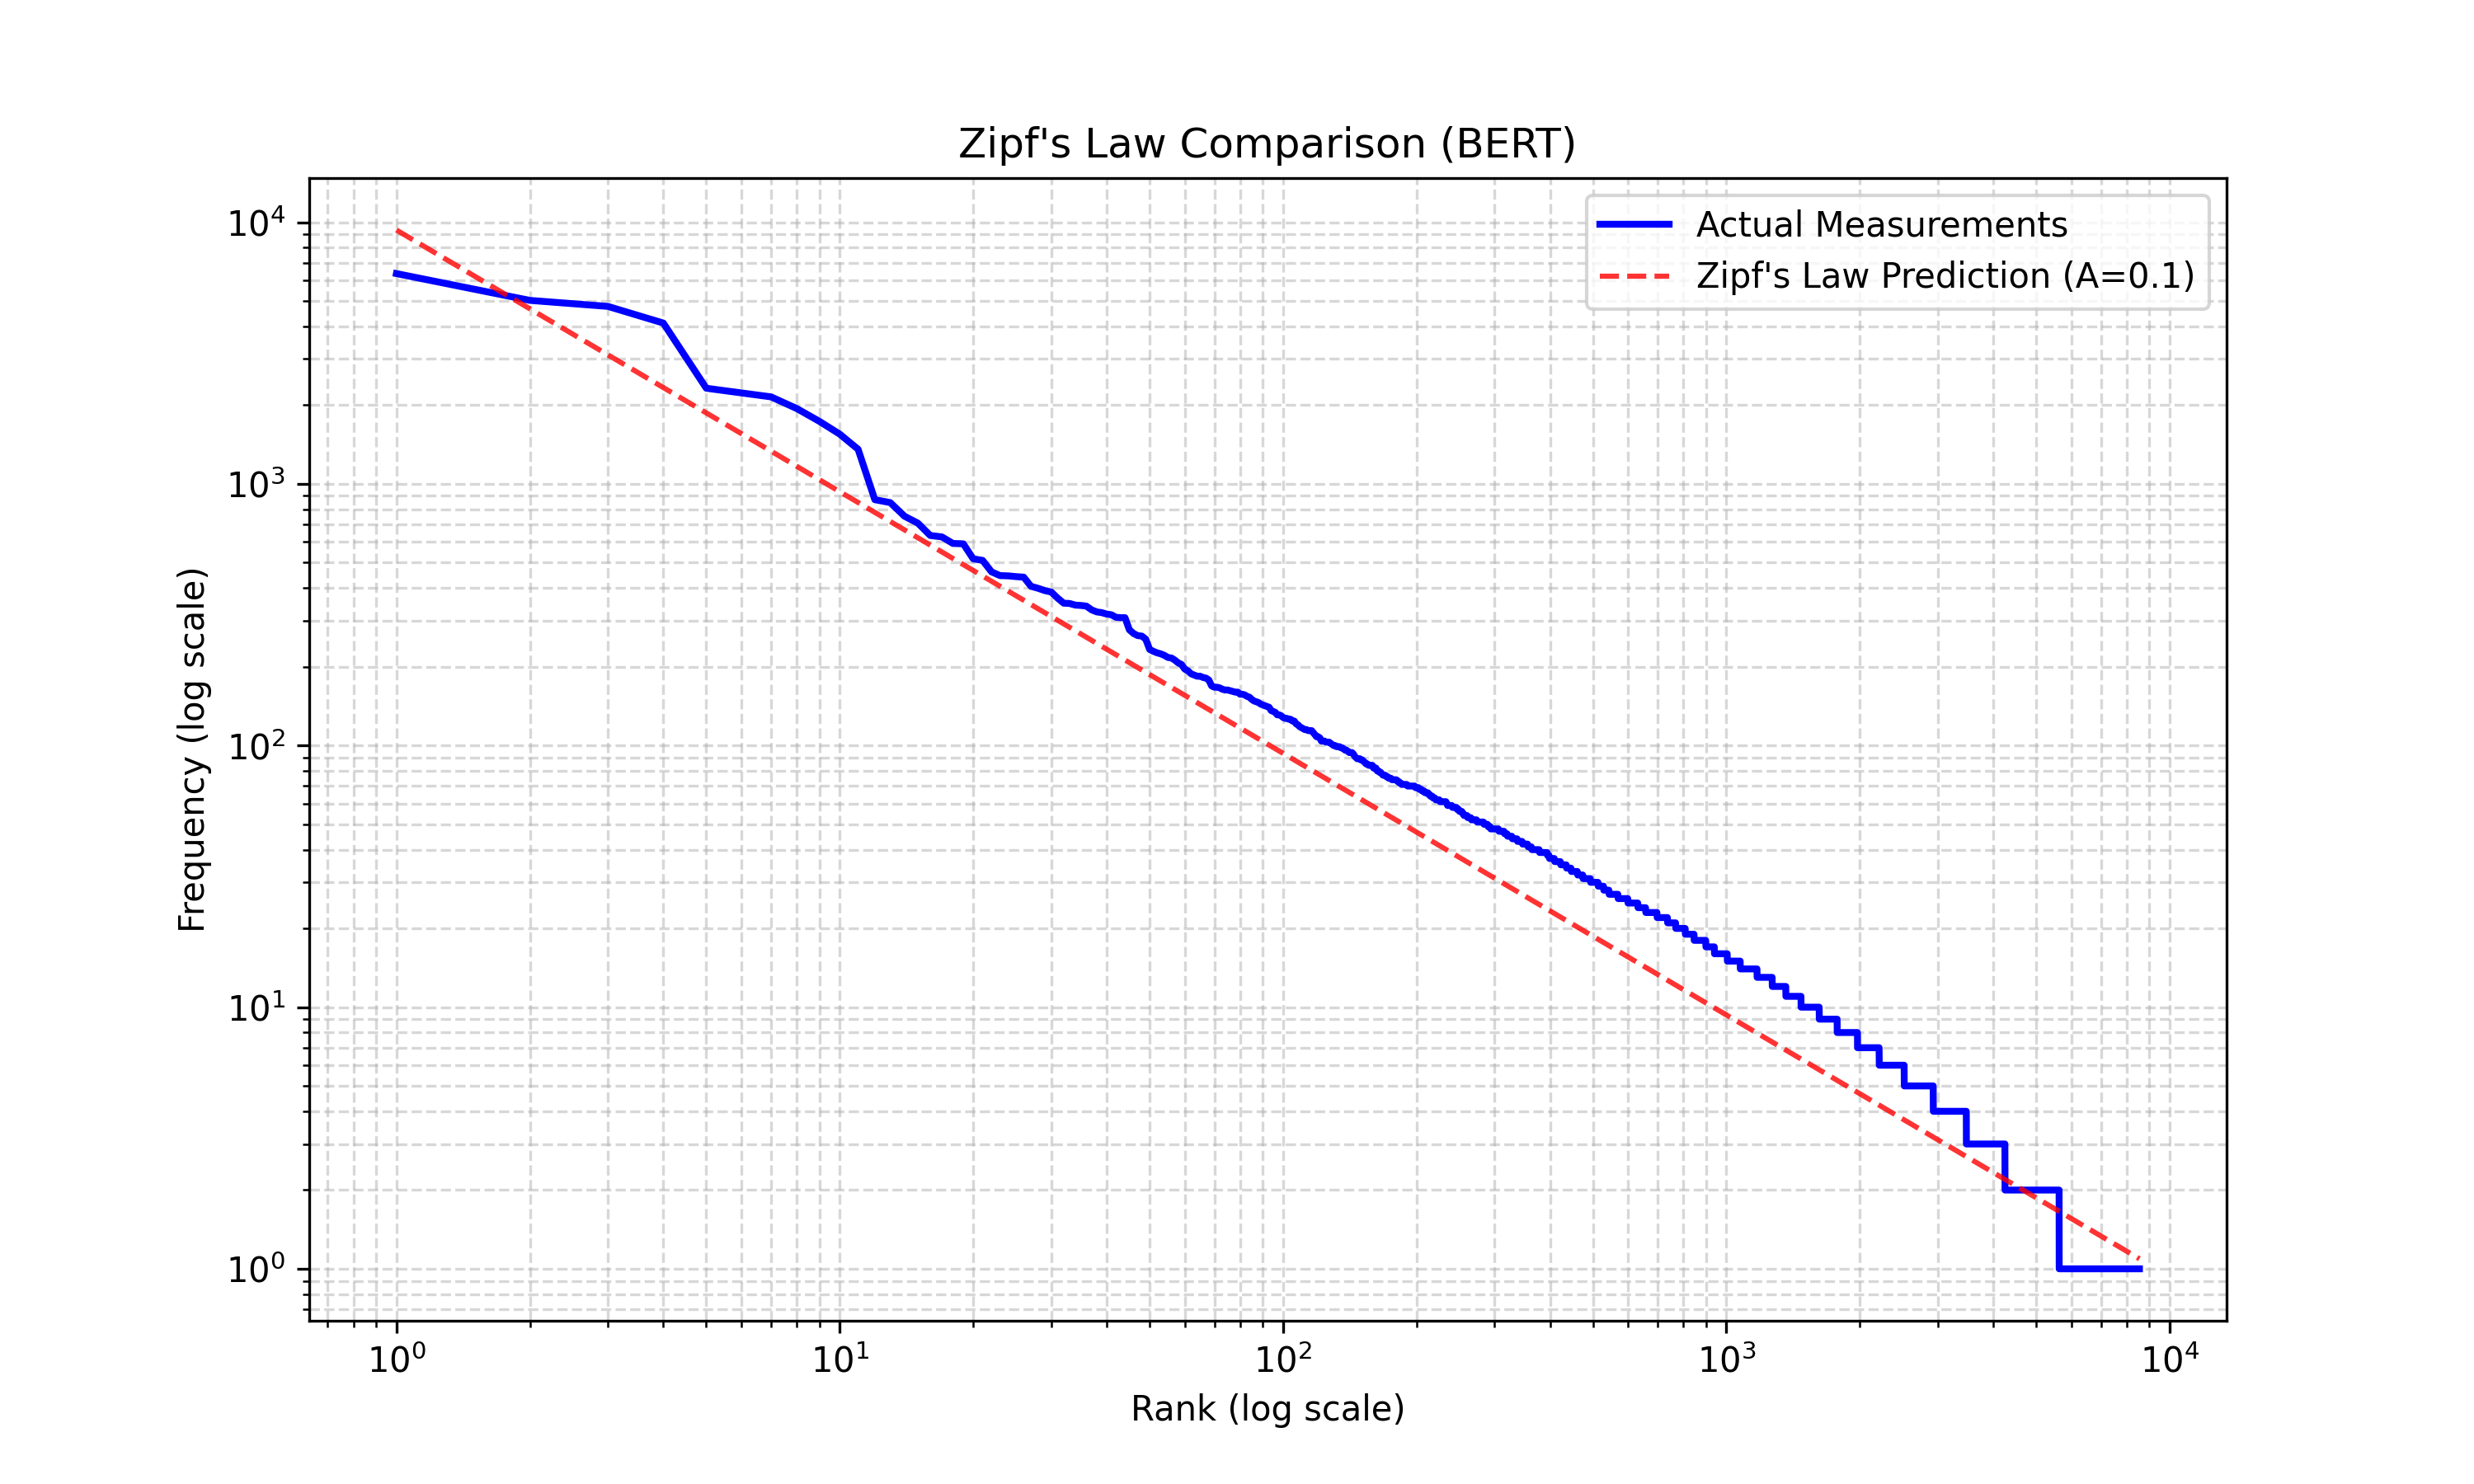
\includegraphics[scale=0.7]{images/bert_zipf_law_comparison.png}
\end{center}

\subsection*{5}


Following is the prompt I used for ChatGPT:


\begin{quote}
``I have the tokens from 3 libraries: NLTK, spaCy and BERT.

Generate Python code for the following assignment:
Σύμφωνα με τον Νόμο του Zipf, το γινόμενο της πιθανότητας ενός type επί την θέση του στη λίστα των types (ταξινομημένη κατά φθίνουσα σειρά συχνότητας) είναι ίσο με μια σταθερά Α. Βρείτε ποια τιμή της σταθεράς A (εξετάστε τις επιλογές: 0.1, 0.2, 0.3, …, 1.0) ταιριάζει καλύτερα με το συγκεκριμένο σύνολο κείμενων. Δημιουργήστε ένα διάγραμμα όπου ο άξονας x είναι η θέση ενός type σε φθίνουσα σειρά συχνότητας και ο άξονας y είναι η συχνότητα του type στην συλλογή. Και οι 2 άξονες να ακολουθούν την λογαριθμική κλίμακα. Δείξτε στο ίδιο διάγραμμα με διαφορετικά χρώματα (i) τις προβλέψεις του νόμου του Zipf (με την καλύτερη τιμή που βρέθηκε για τη σταθερά Α) και (ii) τις πραγματικές μετρήσεις που έγιναν στα κείμενα.

Make sure you generate 2 separate functions: one to find the best A value and another to plot the diagrams. Make sure each function accepts and returns the necessary variables.``

\end{quote}

The generated code is in my report notebook. No changes were necessary to be made.

\section*{B. N-gram Language Models}

\subsection*{1}

\begin{table}[H]
\centering
\begin{tabular}{|c|c|c|c|}
\hline
\multicolumn{1}{|r|}{\textbf{Language model}} & \multicolumn{1}{l|}{\textbf{Original Text}} & \multicolumn{1}{r|}{\textbf{Lowercase}} & \multicolumn{1}{r|}{\textbf{Abstract digits}} \\ \hline
Bigrams (k = 1)                               & 383.738                                     & 591.358                                 & 555.858                                       \\ \hline
Bigrams (k = 0.01)                            & 137.839                                     & 349.178                                 & 274.965                                       \\ \hline
Trigrams (k = 1)                              & 1352.323                                    & 1963.496                                & 1740.481                                      \\ \hline
Trigrams (k = 0.01                            & 429.445                                     & 1024.961                                & 796.219                                       \\ \hline
\end{tabular}
\end{table}

\textbf{Smoothing Parameter (k)}
In each row, $k=0.01$ results in a significantly better (lower) perplexity. The $k=1$ (Laplace) smoothing is too aggressive for this dataset. it reassigns too much probability mass from observed n-grams to unobserved ones, which increases the model's uncertainty (perplexity).

\textbf{Bigrams vs. Trigrams}
Bigrams consistently outperform trigrams in every case. This is expected because our corpus is too small to create a large enough vocabulary of trigram combinations that we encounter in the test dataset. Hence, the models rely on the smoothing fallback during evaluation.

\textbf{Lowecase}
Lowercasing increases perplexity. While it merges word variants (e.g., "The" and "the"), this causes more words to meet the frequency threshold of 3. This reduces the frequency of the ``<UNK>`` token and makes the vocabulary larger. This forces the complicates the model which has to predict specific words instead of assigning ``<UNK>``, thus increasing perplexity.

\textbf{Abstract Digits}
This method shows an increased performance compared to the previous method. Digit abstraction leads to vocabulary shrinkage thus making the model less complex. All digit combinations collapse into a combination of ``\#`` tokens which the model does not have to learn, which leads to reduced complexity.

\subsection*{2}

In general, all models produce mostly incoherent text due to the small vocabulary size. The Trigram models produced much more coherent sentences than the Bigrams.

Sentences generated with k=0.01 were far more realistic. At k=1, the probability distribution is too flat and the model frequently chooses random, unrelated words, resulting in less meaningful sentences.

% \subsection*{References}
% \begin{itemize}
%     \item{NLTK \lstinline{word_tokenize} src: \url{https://github.com/nltk/nltk/blob/develop/nltk/tokenize/__init__.py#L127}}
%     \item{SpaCy tokenizer docs: \url{https://spacy.io/usage/linguistic-features#how-tokenizer-works}}
%     \item{FreqDist from NLTK: \url{https://www.nltk.org/api/nltk.probability.FreqDist.html}}
%     \item{Pandas DF different dict size: \url{https://www.statology.org/pandas-dataframe-from-dict-with-different-length/}}
%     \item{Pandas DF alight text center: \url{https://stackoverflow.com/questions/17232013/how-to-set-the-pandas-dataframe-data-left-right-alignment}}
%     \item{Pandas fix column type: \url{https://pandas.pydata.org/docs/user_guide/integer_na.html}}
%     \item{Set intersection \url{https://www.w3schools.com/python/ref_set_intersection.asp}}
    % \item{List flatten \url{https://stackoverflow.com/questions/952914/how-do-i-make-a-flat-list-out-of-a-list-of-lists}}
        % \item{n-gram perplexity \url{https://medium.com/data-science/implementing-a-character-level-trigram-language-model-from-scratch-in-python-27ca0e1c3c3f}}
        
% \end{itemize}

\end{document}
